\باب{حافظ زاویہ نقشہ کشی}
اگر \عددی{z} سطح میں دائرہ کار \عددی{D} میں مخلوط تفاعل \عددی{w=f(z)} معین ہو، تب \عددی{D} میں ہر نقطہ کا مطابقتی نقطہ \عددی{w} سطح میں پایا جاتا ہے۔یوں \عددی{D}
 کا مطابقتی، \عددی{f(z)} کے حلقہ کا نقشہ، \عددی{w} سطح پر حاصل ہو گا۔جیومیٹریائی نقشہ ذہن میں تفاعل کی تصویر قائم کرتا ہے۔مختلف منحنیات اور خطوں کے نقوش دیکھ کر مخلوط تفاعل سمجھنے میں مدد ملتی ہے۔

جیسا ہم دیکھیں گے، اگر \عددی{f(z)} \ترچھا{تحلیلی} ہو تب \عددی{f(z)} سے حاصل نقشے میں زاویے تبدیل نہیں ہوں گے ماسوائے ان نقطوں پر جہاں \عددی{f'(z)=0} ہو۔ایسا نقشہ \اصطلاح{حافظ زاویہ نقشہ}\فرہنگ{حافظ زاویہ نقشہ}\فرہنگ{نقشہ!حافظ زاویہ}\حاشیہب{conformal map}\فرہنگ{conformal!map}\فرہنگ{mapping!conformal} کہلاتا ہے۔ 

\اصطلاح{حافظ زاویہ نقشہ گشی}\فرہنگ{حافظ زاویہ نقشہ کشی}\حاشیہب{conformal mapping}\فرہنگ{conformal!mapping} کے ذریعہ دیے گیے پیچیدہ خطے کا تبادل سادہ خطے میں کرتے ہوئے نظریہ مخفی قوہ کی دو بعدی سرحدی مسائل حل کیے جاتے ہیں۔اسی وجہ سے حافظ زاویہ نقشہ گشی انجینئری میں اہمیت رکھتی ہے۔

ہم نقشہ گشی کی تعریف پیش کرنے کے بعد نقشہ گشی کا عمل سکھائیں گے۔اس کے بعد کئی بنیادی تحلیلی تفاعل  کے نقوش پیش کریں گے۔

\حصہ{نقشہ گشی}
حقیقی متغیرہ \عددی{x} کے حقیقی تفاعل \عددی{y=f(x)} کی منحنی  کو کارتیسی \عددی{xy} سطح پر  کھینچا جا سکتا ہے۔اس خط کو تفاعل کی \ترچھا{ترسیم} کہتے ہیں۔چونکہ مخلوط متغیرہ \عددی{z} کو جیومیٹریائی طور پر مخلوط سطح میں نقاط سے ظاہر کیا جاتا ہے اور یہی کچھ  \عددی{w} کے لئے بھی درست ہے لہٰذا مخلوط تفاعل
\begin{align}
w=f(z)=u(x,y)+iv(x,y)\quad \quad \quad (z=x+iy)
\end{align}
کی صورت حال زیادہ پیچیدہ ہے۔اس سے ہمیں خیال آتا ہے کہ ہم ان دو متغیرات کے لئے دو علیحدہ علیحدہ مخلوط سطحیں استعمال کریں۔ایک \عددی{z} سطح جس میں \عددی{z=x+iy} دکھایا جائے اور دوسری \عددی{w} سطح جس میں مطابقتی \عددی{w=u+iv} دکھایا جائے۔یوں  \عددی{f(z)} کی دائرہ کار \عددی{D} میں ہر \عددی{z}  کے لئے تفاعل \عددی{f(z)}  سطح \عددی{w}   میں قیمت \عددی{w=f(z)}  مختص کرے گا۔اس معین تعلق کو \عددی{f} کی دائرہ کار کی سطح \عددی{w} \اصطلاح{میں}\فرہنگ{میں}\حاشیہب{into}\فرہنگ{into}  \اصطلاح{نقشہ گشی}\فرہنگ{نقشہ گشی}\حاشیہب{mapping}\فرہنگ{mapping} (یا \ترچھا{تبادل}) کہتے ہیں، یا \عددی{f} کی دائرہ کار کا \عددی{f} کے حلقہ \اصطلاح{پر}\فرہنگ{پر}\حاشیہب{onto}\فرہنگ{onto} نقشہ کشی کہتے ہیں۔

\عددی{w_0=f(z_0)} جو نقطہ \عددی{z_0} کا مطابقتی نقطہ ہے،  \عددی{f(z)} کے لحاظ سے نقشے میں، \عددی{z_0} کا  \اصطلاح{عکس نقطہ}\فرہنگ{عکس نقطہ}\حاشیہب{image point}\فرہنگ{image!point} یا \اصطلاح{عکس}\فرہنگ{عکس}\حاشیہب{image}\فرہنگ{image} کہلاتا ہے۔ اگر \عددی{z} کسی منحنی پر حرکت کرے اور \عددی{f(z)} استمراری (نا کہ مستقل)  ہو تب مطابقتی نقطہ \عددی{w=f(z)} عمومی طور پر سطح \عددی{w} میں منحنی \عددی{C^*} پر حرکت کرے گا۔اس منحنی کو منحنی \عددی{C} کا عکس کہیں گے۔لفظ "عکس" کسی بھی نقطوں کے سلسلے اور خطہ کے لئے بھی استعمال کیا جاتا ہے۔ 

ہم دیکھیں گے کہ ایسی نقشہ کشی کی خواص کی تفتیش،  \عددی{z} سطح میں منحنیات اور خطے اور  \عددی{w} سطح میں ان کے عکس پر غور اور \عددی{w} سطح میں منحنیات اور خطے اور  \عددی{z} سطح میں ان کے عکس پر غور  کرنے سے  کی جا سکتی ہے۔ اس طرح  انفرادی نقطوں پر غور کرنے سے حاصل معلومات سے  زیادہ معلومات حاصل ہو گی۔

اگرچہ  \عددی{w} اور \عددی{z} کو دو علیحدہ علیحدہ سطحوں سے ظاہر کیا جاتا ہے، بعض اوقات یوں  سوچنا زیادہ بہتر ثابت ہوتا ہے  کہ اصل اور نقش ایک ہی سطح پر پائے جاتے ہوں اور  عمومی اصطلاحات مثلاً " گھومنا" اور "مستقیم حرکت" استعمال کرنا۔یوں \عددی{w=z+3}   مستقیم حرکت کہلائے گی جو \عددی{z} سطح میں ہر نقطہ کو دائیں جانب تین اکایاں منتقل کرتی ہے۔

تحلیل تفاعل \عددی{w=u+iv=f(z)} جس نقشہ کو ظاہر کرتا ہو، کی کسی مخصوص  خاصیت  جاننے کے لئے ہم \عددی{z} سطح میں سیدھے لکیروں \عددی{x=\text{مستقل}} اور \عددی{y=\text{مستقل}} کا \عددی{w} سطح میں عکس پر غور کر سکتے ہیں۔اسی طرح ہم دائرہ \عددی{\abs{z}=\text{مستقل}} یا مبدا سے گزرتی سیدھی لکیروں کی عکس پر غور کر سکتے ہیں۔اس کے علاوہ ہم \عددی{u(x,y)=\text{مستقل}} اور \عددی{v(x,y)=\text{مستقل}} منحنیات پر \عددی{z} سطح میں غور کر سکتے ہیں۔ان منحنیات کو \عددی{u} اور \عددی{v} کی \اصطلاح{ہموار منحنیات}\فرہنگ{ہموار!منحنی}\حاشیہب{level curves}\فرہنگ{curve!level} کہتے ہیں۔ ہم سادہ اشکال مثلاً چکور، تکون، مستطیل وغیرہ اور ان کے عکس پر بھی غور کر سکتے ہیں۔

آئیں چند مثالوں کی مدد سے ان حقائق کو بہتر سمجھنے کی کوشش کرتے ہیں۔

%====================
\ابتدا{مثال}\شناخت{مثال_نقش_خطی_مستقیم}\quad \موٹا{خطی تبادل \عددی{w=ax+b}}\\
درج ذیل نقش \اصطلاح{مستقیم حرکت} کو ظاہر کرتا ہے۔
\begin{align}\label{مساوات_نقش_خطی_مستقیم_الف}
w=z+b
\end{align}
شکل \حوالہ{شکل_مثال_نقش_خطی_مستقیم} میں مساوات \حوالہ{مساوات_نقش_خطی_مستقیم_الف} کو \عددی{w=z+2+i} کے لئے دکھایا گیا ہے جہاں مستطیل اور اس کا عکس دکھائے گئے ہیں جو یکساں ہیں (کیوں؟)۔\عددی{A} کا عکس \عددی{A^*}، وغیرہ۔زیادہ پیچیدہ اشکال میں نقطوں کو اس طرح ظاہر کرنا مفید ثابت ہوتا ہے۔ مساوات \حوالہ{مساوات_نقش_خطی_مستقیم_الف} میں \عددی{b=0} پر کرنے سے \اصطلاح{مماثل تبادل}\فرہنگ{تبادل!مماثل}\حاشیہب{identity transformation}\فرہنگ{transformation!identity} 
\begin{align*}
w=z
\end{align*}
حاصل ہوتا ہے جو ہر نقطے کو اپنے آپ پر نقش کرتا ہے۔
%
\begin{figure}
\centering
\begin{tikzpicture}
\draw(0,0)--++(3,0)node[below]{$x$};
\draw(0,0)node[below]{$0$}--++(0,2)node[right]{$y$};
\draw(1,0.5)node[left]{$A$}--++(0.5,0)node[right]{$B$}--++(0,1)node[right]{$C$}--++(-0.5,0)node[left]{$D$}--++(0,-1);
\foreach \x in {0.5,1,1.5,2,2.5}{\draw (\x,0)--++(0,0.1);}
\foreach \y in {0.5,1,1.5}{\draw (0,\y)--++(0.1,0);}
\draw(2,0)node[below]{$4$};
\draw(0,1)node[left]{$2$};
\draw(1.5,-0.5)node[below]{\text{\RL{($\,z$ مستوی)}}};
\begin{scope}[shift={(4cm,0)}]
\draw(0,0)--++(3,0)node[below]{$u$};
\draw(0,0)node[below]{$0$}--++(0,2)node[right]{$v$};
\draw(2,1)node[left]{$A^*$}--++(0.5,0)node[right]{$B^*$}--++(0,1)node[right]{$C^*$}--++(-0.5,0)node[left]{$D^*$}--++(0,-1);
\foreach \x in {0.5,1,1.5,2,2.5}{\draw (\x,0)--++(0,0.1);}
\foreach \y in {0.5,1,1.5}{\draw (0,\y)--++(0.1,0);}
\draw(2,0)node[below]{$4$};
\draw(0,1)node[left]{$2$};
\draw(1.5,-0.5)node[below]{\text{\RL{($\,w$ مستوی)}}};
\end{scope}
\end{tikzpicture}
\caption{مستقیم حرکت \عددی{w=z+2+i}}
\label{شکل_مثال_نقش_خطی_مستقیم}
\end{figure}

درج ذیل تبادل
\begin{align*}
w=az\quad \quad \quad (\abs{a}=1)
\end{align*}
مقررہ زاویہ \عددی{\phase{a}} سے گھومنے کو ظاہر کرتا ہے۔شکل \حوالہ{شکل_نقش_گھومنا} میں \عددی{w=iz} یعنی  گھڑی کی سوئیوں کی گھومنے کی الٹ رخ \عددی{\tfrac{\pi}{2}} زاویہ سے گھومنا دکھایا گیا ہے۔
\begin{figure}
\centering
\begin{tikzpicture}
\draw(0,0)--++(3,0)node[below]{$x$};
\draw(0,0)node[below]{$0$}--++(0,2.5)node[right]{$y$};
\draw([shift={(0:1)}]0,0) arc (0:90:1);
\draw([shift={(0:2)}]0,0) arc (0:90:2);
\draw[dashed](0,0)--++(30:2.5);
\draw[dashed](0,0)--++(60:2.5);
\foreach \x in {0.5,1,1.5,2,2.5}{\draw(\x,0)--++(0,0.1);}
\foreach \y in {0.5,1,1.5,2}{\draw(0,\y)--++(0.1,0);}
\draw(2.5,0)node[below]{$5$};
\draw(0,1.5)node[left]{$3$};
\draw(1,0)node[below]{$A$};
\draw(2,0)node[below]{$B$};
\draw(0,1)node[left]{$C$};
\draw(0,2)node[left]{$D$};
\draw(1.5,-0.5)node[below]{\text{\RL{($\,z$ مستوی)}}};
%
\begin{scope}[xshift={8cm}]
\draw(-3,0)--(0.75,0)node[below]{$u$};
\draw(0,0)node[below]{$0$}--++(0,2.5)node[right]{$v$};
\draw([shift={(90:1)}]0,0) arc (90:180:1);
\draw([shift={(90:2)}]0,0) arc (90:180:2);
\draw[dashed](0,0)--++(120:2.5);
\draw[dashed](0,0)--++(150:2.5);
\foreach \x in {0.5,-0.5,-1,-1.5,-2,-2.5}{\draw(\x,0)--++(0,0.1);}
\foreach \y in {0.5,1,1.5,2}{\draw(0,\y)--++(0.1,0);}
\draw(-2.5,0.1)node[above]{$-5$};
\draw(0.1,1.5)node[right]{$3$};
\draw(0,1)node[right]{$A^*$};
\draw(0,2)node[right]{$B^*$};
\draw(-1,0)node[below]{$C^*$};
\draw(-2,0)node[below]{$D^*$};
\draw(-1.5,-0.5)node[below]{\text{\RL{($\,w$ مستوی)}}};
\end{scope}
\end{tikzpicture}
\caption{گھڑی کی الٹ رخ گھومنے کا زاویہ \عددی{\tfrac{\pi}{2}} ہے۔}
\label{شکل_نقش_گھومنا}
\end{figure}

درج ذیل تبادل
\begin{align*}
w=az \quad \quad \quad (\text{\RL{مثبت حقیقی $a$}})
\end{align*}
میں \عددی{a>1} اتساع جبکہ \عددی{0<a<1} سکڑاو کو ظاہر کرتا ہے۔اسی طرح 
\begin{align}
w=az\quad \quad \quad (\text{\RL{اختیاری $a$}})
\end{align}
زاویہ \عددی{\phase{a}} سے گھومنے کو اور ساتھ ہی یکساں اتساع یا سکڑاو کو ظاہر کرتا ہے۔ درج ذیل تبادل
\begin{align}
w=az+b
\end{align}
\اصطلاح{خطی تبادل}\فرہنگ{تبادل!خطی}\حاشیہب{linear transformation}\فرہنگ{transformation!linear} کہلاتا ہے جو گھومنے کے ساتھ اتساع یا سکڑاو \عددی{w_1=az} کے ساتھ ساتھ مستقیم حرکت \عددی{w=w_1+b} کو ظاہر کرتا ہے۔ شکل \حوالہ{شکل_نقش_خطی_تبادل} میں \عددی{w=(1+i)z+2i} تبادل دکھایا گیا ہے جو گھڑی کی الٹ رخ  \عددی{\tfrac{\pi}{4}} زاویے کے گھومنے اور \عددی{\abs{1+i}=\sqrt{2}} تناسب کی اتساع کے بعد اوپر کی رخ مستقیم حرکت کو ظاہر کرتا ہے۔  
\begin{figure}
\centering
\begin{tikzpicture}
\draw(0,0)--++(2,0)node[below]{$x$};
\draw(0,0)--++(0,2)node[left]{$y$};
\draw([shift={(0:0.5)}]0,0) arc (0:90:0.5);
\draw([shift={(0:1)}]0,0) arc (0:90:1);
\draw([shift={(0:1.5)}]0,0) arc (0:90:1.5);
\draw(0.5,0)node[below]{$1$};
\draw(1,0)node[below]{$2$};
\draw(1.5,0)node[below]{$3$};
\draw(0,0.5)node[left]{$1$};
\draw(0,1)node[left]{$2$};
\draw(0,1.5)node[left]{$3$};
\draw[thick](0,0)--++(1.5,0)node[shift={(0.2,0.2)}]{$B$};
\draw[thick](0,0)node[shift={(0.2,0.2)}]{$A$}--++(0,1.5)node[shift={(0.2,0.2)}]{$C$};
\draw(1,-1)node[]{$z=x+iy$};
\draw(1,-1.5)node[]{\text{\RL{($\,z$ مستوی)}}};
\draw(0,0)node[below]{$0$}node[left]{$0$};
\begin{scope}[xshift={(4cm)}]
\draw(-1.5,0)--(1.5,0)node[below]{$u_1$};
\draw(0,0)--++(0,2.75)node[right]{$v_1$};
\draw([shift={(45:0.707)}]0,0) arc (45:135:0.707);
\draw([shift={(45:1.4142)}]0,0) arc (45:135:1.4142);
\draw([shift={(45:2.121)}]0,0) arc (45:135:2.121);
\draw(0,0)node[below]{$0$};
\draw[thick](0,0)node[shift={(0.5,0.2)}]{$A^*$}--++(45:2.212)node[right]{$B^*$};
\draw[thick](0,0)--++(135:2.212)node[left]{$C^*$};
\foreach \x in {-1,-0.5,1}{\draw(\x,0)--++(0,0.1);}
\foreach \y in {0.5,1,1.5,2,2.5}{\draw(0,\y)--++(0.1,0);}
\draw(0,2.5)node[left]{$5$};
\draw(1,-1)node[]{$w_1=u_1+iv_1$};
\draw(1,-1.5)node[]{\text{\RL{($\,w_1$ مستوی)}}};
\end{scope}
\begin{scope}[xshift={(8cm)}]
\draw(-1.5,0)--(1.5,0)node[below]{$u$};
\draw(0,0)--++(0,3.75)node[right]{$v$};
\draw([shift={(45:0.707)}]0,1) arc (45:135:0.707);
\draw([shift={(45:1.4142)}]0,1) arc (45:135:1.4142);
\draw([shift={(45:2.121)}]0,1) arc (45:135:2.121);
\draw(0,0)node[below]{$0$};
\draw[thick](0,1)node[shift={(0.5,0.2)}]{$A^{**}$}--++(45:2.212)node[right]{$B^{**}$};
\draw[thick](0,1)--++(135:2.212)node[left]{$C^{**}$};
\foreach \x in {-1,-0.5,0.5,1}{\draw(\x,0)--++(0,0.1);}
\foreach \y in {0.5,1,1.5,2,2.5,3.5}{\draw(0,\y)--++(0.1,0);}
\draw(0,2.6)node[left]{$5$};
\draw(1,-1)node[]{$w=u+iv$};
\draw(1,-1.5)node[]{\text{\RL{($\,w$ مستوی)}}};
\end{scope}
\end{tikzpicture}
\caption{خطی تبادل $w=(1+i)z+2i$ جس میں  گھومنا،  اتساع $w_1=(1+i)z$ اور مستقیم حرکت $w=w_1+2i$ شامل ہے۔}
\label{شکل_نقش_خطی_تبادل}
\end{figure}
\انتہا{مثال}
%========================
\ابتدا{مثال}\quad \موٹا{نقش \عددی{w=z^2}}\\
ہم درج ذیل نقش پر غور کرنا چاہتے ہیں۔
\begin{align}\label{مساوات_نقش_مربع_الف}
w=z^2
\end{align}
یہاں قطبی محدد استعمال کرنا بہتر ثابت ہوتا ہے۔یوں \عددی{z=e^{i\theta}} اور \عددی{w=Re^{i\phi}} لیتے ہوئے  مساوات \حوالہ{مساوات_نقش_مربع_الف} \عددی{Re^{i\phi}=r^2e^{i2\theta}} لکھی جائے گی جس سے 
\begin{align*}
R=r^2,\quad \phi=2\theta
\end{align*}
حاصل ہوتے ہیں۔ یوں دائروں \عددی{r=r_0=\text{مستقل}} کا نقش دائرے \عددی{R=r_0^2=\text{مستقل}} ہوں گے جبکہ مبدا سے گزرتی سیدھی لکیروں \عددی{\theta=\theta_0=\text{مستقل}} کا نقش دگنی زاویہ پر لکیریں \عددی{\phi=2\theta_0=\text{مستقل}} ہوں گی۔ خاص کر \عددی{z} سطح میں مثبت حقیقی محور \عددی{(\theta=0)} کا نقش \عددی{w} سطح میں مثبت حقیقی محور ہو گا جبکہ \عددی{z} سطح میں مثبت خیالی محور \عددی{\theta=\tfrac{\pi}{2}} کا نقش \عددی{w} سطح میں منفی حقیقی محور ہو گا۔ یہ نقش  مبدا پر ہر زاویہ کو دگنا کرتا ہے۔ربع اول \عددی{0\le \theta \le \tfrac{\pi}{2}} کا نقش بالائی نصف \عددی{w} سطح ہو گی (شکل \حوالہ{شکل_نقش_مربع})۔
\begin{figure}
\centering
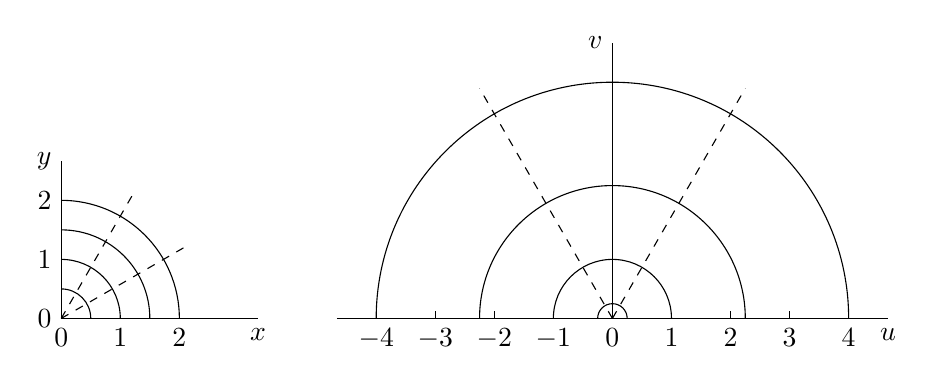
\begin{tikzpicture}
\pgfmathsetmacro{\len}{3/4}
\draw(0,0)--++(2.5,0)node[below]{$x$};
\draw(0,0)--++(0,2)node[left]{$y$};
\draw([shift={(0:0.5*\len)}]0,0) arc (0:90:0.5*\len);
\draw([shift={(0:1*\len)}]0,0) arc (0:90:1*\len);
\draw([shift={(0:1.5*\len)}]0,0) arc (0:90:1.5*\len);
\draw([shift={(0:2*\len)}]0,0) arc (0:90:2*\len);
\draw(1*\len,0)node[below]{$1$};
\draw(2*\len,0)node[below]{$2$};
\draw(0,1*\len)node[left]{$1$};
\draw(0,2*\len)node[left]{$2$};
\draw[dashed](0,0)--++(30:2.5*\len);
\draw[dashed](0,0)node[below]{$0$}node[left]{$0$}--++(60:2.5*\len);
\begin{scope}[xshift={(7cm)}]
\draw(-3.5,0)--(3.5,0)node[below]{$u$};
\draw(0,0)--++(0,3.5)node[left]{$v$};
\draw([shift={(0:0.25*\len)}]0,0) arc (0:180:0.25*\len);
\draw([shift={(0:1*\len)}]0,0) arc (0:180:1*\len);
\draw([shift={(0:2.25*\len)}]0,0) arc (0:180:2.25*\len);
\draw([shift={(0:4*\len)}]0,0) arc (0:180:4*\len);
\foreach \x in {-3,-2,2,3}{\draw(\x*\len,0)--++(0,0.1);}
\draw(1*\len,0)node[below]{$1$};
\draw(2*\len,0)node[below]{$2$};
\draw(3*\len,0)node[below]{$3$};
\draw(4*\len,0)node[below]{$4$};
\draw(-1*\len,0)node[below]{$-1$};
\draw(-2*\len,0)node[below]{$-2$};
\draw(-3*\len,0)node[below]{$-3$};
\draw(-4*\len,0)node[below]{$-4$};
\draw[dashed](0,0)node[below]{$0$}--++(60:4.5*\len);
\draw[dashed](0,0)--++(120:4.5*\len);
\end{scope}
\end{tikzpicture}
\caption{نقش \عددی{w=z^2}}
\label{شکل_نقش_مربع}
\end{figure}

مستطیل محدد میں تبادل \عددی{w=z^2} درج ذیل دے گا۔
\begin{align*}
u+iv=x^2-y^2+i2xy
\end{align*}
حقیقی اور خیالی اجزاء علیحدہ کرتے ہوئے 
\begin{align}\label{مساوات_نقش_مربع_ب}
u=x^2-y^2,\quad v=2xy
\end{align}
ملتا ہے۔ہم دیکھتے ہیں کہ \عددی{u} اور \عددی{v} کی \اصطلاح{ہموار سطحات}\فرہنگ{ہموار!سطح}\فرہنگ{سطح!ہموار} متساوی الاضلاع قطع زائد ہوں گے جن کی متقارب لکیریں\فرہنگ{متقارب!لکیریں}\حاشیہب{asymptotes} \عددی{y=\mp x} اور محدد کی محور ہیں۔ہم دیکھتے ہیں مساوات \حوالہ{مساوات_نقش_مربع_ب} میں دیے گئے  خطوط ایک دوسرے کی عمودی مطقاطع خطوط (حصہ \حوالہ{حصہ_درجہ_اول_عمودی_خطوط_کی_نسلیں}) ہیں۔ شکل \حوالہ{شکل_نقش_مربع_ہموار_سطحیں} میں \عددی{z} سطح میں دو خطے \عددی{w} سطح میں مستطیل پر نقش ہوں گے۔ظاہر ہے کہ ہر نقطہ \عددی{w\ne 0} سطح \عددی{z} میں ٹھیک  دو نقطوں کا عکس ہو گا۔

ہم مساوات \حوالہ{مساوات_نقش_مربع_ب} استعمال کرتے ہوئے سیدھی خطوط \عددی{x=\text{مستقل}} اور \عددی{y=\text{مستقل}} کا عکس تلاش کر سکتے ہیں۔خط \عددی{x=c=\text{مستقل}} کا عکس
\begin{align*}
u=c^2-y^2,\quad v=2cy
\end{align*}
سے \عددی{y} حذف کرتے ہوئے
\begin{align*}
v^2=4c^2(c^2-u)
\end{align*}
حاصل ہوتا ہے جو قطع مکافی کو ظاہر کرتی ہے جو بائیں رخ کھلتا ہے۔مبدا اس قطع مکافی کا ماسکہ ہو گا۔اسی طرح \عددی{y=k=\text{مستقل}} کا عکس
\begin{align*}
v^2=4k^2(k^2+u)
\end{align*}
ہو گا جو دائیں کو کھلتا ہوا قطع مکافی ہے جس کا ماسکہ عین مبدا پر ہے (شکل \حوالہ{شکل_نقش_مربع_نقش_میں_سیدھے_خطوط_کا_عکس})۔
\begin{figure}
\centering
\begin{tikzpicture}
\begin{axis}[small,clip=false,axis lines*=middle,ymin=-3,ymax=3,xmin=-3,xmax=3.5,xtick={-1,1},ytick={-1,1},xticklabels={$-1$,$1$},yticklabels={$-1$,$1$},xlabel={$x$},ylabel={$y$},ylabel style={rotate=-90},xlabel style={at={(current axis.right of origin)},anchor=west},ylabel style={at={(current axis.above origin)},anchor=south}]
\shade[fill=gray!20!white](axis cs: 1.53,0.64)--(axis cs:1.7989,1.1118)--(axis cs: 2.236,0.8944)--(axis cs:2.05817,0.4858)--(axis cs: 1.53,0.64);
\shade[fill=gray!20!white](axis cs: 2.236,0.8944)--(axis cs:2.05817,0.4858)--(axis cs:2.48239,0.402837)--(axis cs:2.57,0.7782)--(axis cs:2.236,0.8944);
%
\shade[fill=gray!20!white](axis cs: -1.53,-0.64)--(axis cs:-1.7989,-1.1118)--(axis cs: -2.236,-0.8944)--(axis cs:-2.05817,-0.4858)--(axis cs: -1.53,-0.64);
\shade[fill=gray!20!white](axis cs: -2.236,-0.8944)--(axis cs:-2.05817,-0.4858)--(axis cs:-2.48239,-0.402837)--(axis cs:-2.57,-0.7782)--(axis cs:-2.236,-0.8944);
%
\addplot[domain=-2:2]{sqrt(x^2-0)}node[pin=30:{$u=0$}]{};
\addplot[domain=-2:2,name path=ut]{sqrt(x^2+2)};
\addplot[domain=-2:2,name path=uf]{sqrt(x^2+4)};
\addplot[domain=-2:2]{sqrt(x^2+6)}node[pin=30:{$u=-6$}]{};
%
\addplot[domain=-2:2]{-sqrt(x^2-0)};
\addplot[domain=-2:2]{-sqrt(x^2+2)};
\addplot[domain=-2:2]{-sqrt(x^2+4)};
\addplot[domain=-2:2]{-sqrt(x^2+6)};
%
\addplot[domain=-2:2]({sqrt(2+x^2)},{x});
\addplot[domain=-2:2]({sqrt(4+x^2)},{x});
\addplot[domain=-2:2]({sqrt(6+x^2)},{x})node[pin=0:{$u=6$}]{};
%
\addplot[domain=-2:2]({-sqrt(2+x^2)},{x});
\addplot[domain=-2:2]({-sqrt(4+x^2)},{x});
\addplot[domain=-2:2]({-sqrt(6+x^2)},{x});
%%
\addplot[domain=0.35:3,dashed,name path=vt]({x},{2/(2*x)})node[pin={[pin edge=solid]0:{$v=2$}}]{};
\addplot[domain=0.7:3,dashed,name path=vf]({x},{4/(2*x)});
\addplot[domain=1.05:3,dashed]({x},{6/(2*x)})node[pin={[pin edge=solid]0:{$v=6$}}]{};
%
\addplot[domain=0.35:3,dashed]({x},{-2/(2*x)});
\addplot[domain=0.7:3,dashed]({x},{-4/(2*x)});
\addplot[domain=1.05:3,dashed]({x},{-6/(2*x)})node[solid,pin={[pin distance=0.25cm,pin edge=solid]0:{$v=-6$}}]{};
%
\addplot[domain=0.35:3,dashed](-{x},{2/(2*x)});
\addplot[domain=0.7:3,dashed](-{x},{4/(2*x)});
\addplot[domain=1.05:3,dashed](-{x},{6/(2*x)});
%
\addplot[domain=0.35:3,dashed](-{x},{-2/(2*x)});
\addplot[domain=0.7:3,dashed](-{x},{-4/(2*x)});
\addplot[domain=1.05:3,dashed](-{x},{-6/(2*x)});
\end{axis}
\begin{scope}[shift={(8cm,2cm)}]
\pgfmathsetmacro{\kk}{0.25}
\draw[dashed](-4.5*\kk,0)--(4.5*\kk,0)node[right]{$u$};
\draw(0,-4.5*\kk)--(0,4.5*\kk)node[above]{$v$};
%
\shade[gray!20!white](1*\kk,1*\kk)--++(2*\kk,0)--++(0,1*\kk)--++(-2*\kk,0)--++(0,-1*\kk);
%
\foreach \x in {-4,-3,-2,-1,1,2,3,4}{\draw(\x*\kk,-4.5*\kk)--++(0,9*\kk);}
\foreach \y in {-4,-3,-2,-1,1,2,3,4}{\draw[dashed](-4.5*\kk,\y*\kk)--++(9*\kk,0);}
\draw(0,0)node[ocirc]{};
\end{scope}
\end{tikzpicture}
\caption{نقش $w=z^2$ کی صورت میں $u$ اور $v$ کی ہموار سطحیں}
\label{شکل_نقش_مربع_ہموار_سطحیں}
\end{figure}
%
\begin{figure}
\centering
\begin{tikzpicture}
\begin{axis}[small,clip=false,axis lines*=middle,ymin=-5,ymax=5,xmin=-5.5,xmax=5.5,xtick={-2,-3,-5,2,3,5},xticklabels={$-2$,$-3$,$-5$,$2$,$3$,$5$},ytick={-4,-2,2,4},yticklabels={$-4$,$-2$,$2$,$4$},xlabel style={at={(current axis.right of origin)},anchor=west},ylabel style={rotate=-90},ylabel style={at={(current axis.above origin)},anchor=west},xlabel={$u$},ylabel={$v$}]
\addplot[dashed,domain=-2.3:2.3] ({0.5^2-x^2/(4*0.5^2)},{x})node[pos=0,left]{$x=\tfrac{1}{2}$};
\addplot[dashed,domain=-5:5] ({1^2-x^2/(4*1^2)},{x})node[pos=0,left]{$x=1$};
\addplot[dashed,domain=-3.5:3.5] ({1.5^2-x^2/(4*1.5^2)},{x});
\addplot[dashed,domain=-5:5] ({2^2-x^2/(4*2^2)},{x})node[pos=0,below]{$x=2$};
%
\addplot[domain=-2.2:2.2] ({x^2/(4*0.5^2)-0.5^2},{x})node[right]{$y=\tfrac{1}{2}$};
\addplot[smooth,domain=-4.5:4.5] ({x^2/(4*1^2)-1^2},{x})node[right]{$y=1$};
\addplot[domain=-3.6:3.6] ({x^2/(4*1.5^2)-1.5^2},{x});
\addplot[domain=-4.5:4.5] ({x^2/(4*2^2)-2^2},{x})node[above]{$y=2$};
\end{axis}
\end{tikzpicture}
\caption{نقش $w=z62$ میں سیدھے خطوط $x=c$ اور $y=c^*$ کے عکس}
\label{شکل_نقش_مربع_نقش_میں_سیدھے_خطوط_کا_عکس}
\end{figure}
\انتہا{مثال}
%===========================
باقی طاقت
\begin{align}
w=z^n,\quad n=3,4,\cdots
\end{align}
پر بھی اسی طرح غور کیا جا سکتا ہے۔ظاہر ہے کہ ان کی ہموار سطحات کی مساوات مزید پیچیدہ ہوں گی۔زاویائی خطہ \عددی{0\le \phase{z} \le \tfrac{\pi}{n}} بالائی نصف \عددی{w} سطح پر نقش ہو گا (شکل \حوالہ{شکل_نقش_عمومی_طاقت})۔

منفی طاقت کی نقش \عددی{\tfrac{1}{z},\tfrac{1}{z^2},\cdots} پر بھی قطبی محدد کی مدد سے غور کیا جا سکتا ہے۔عملاً اہم ترین صورت درج ذیل مثال میں دی گئی ہے۔
\begin{figure}
\centering
\begin{tikzpicture}
\draw(0,0)--++(2,0)node[below]{$x$};
\draw(0,0)--++(0,1)node[left]{$y$};
\draw(0,0)--++(30:1.5);
\draw[-stealth]([shift={(0:0.5)}]0,0) arc (0:30:0.5);
\draw(15:0.9)node{$\tfrac{\pi}{n}$};
%
\begin{scope}[xshift={(6cm)}]
\draw(-2,0)--(2,0)node[below]{$u$};
\draw(0,0)--++(0,1)node[right]{$v$};
\end{scope}
\end{tikzpicture}
\caption{نقش $w=z^n\,$}
\label{شکل_نقش_عمومی_طاقت}
\end{figure}

%=========================
\ابتدا{مثال}\quad \موٹا{نقش $w=\tfrac{1}{z}$۔ الٹ جانا}\\
ہم درج ذیل نقش پر غور کرتے ہیں۔
\begin{align}\label{مساوات_نقش_الٹ_جانا_الف}
w=\frac{1}{z}\quad \quad \quad z\ne 0
\end{align}
قطبی محدد استعمال کرتے ہوئے \عددی{z=re^{i\theta}} اور \عددی{w=Re^{i\phi}} لکھتے ہیں۔یوں مساوات \حوالہ{مساوات_نقش_الٹ_جانا_الف} سے
\begin{align}
R=\frac{1}{r},\quad \phi=-\theta\quad \quad \quad (r\ne 0)
\end{align}
حاصل ہوتا ہے۔اس سے ہم دیکھتے ہیں کہ نقطہ \عددی{w=\tfrac{1}{z}\,(z\ne 0)}، مبدا سے نکلتی سیدھی لکیر جو \عددی{\bar{z}} سے گزرتی ہو پر واقع ہے۔مبدا سے اس نقطے کا فاصلہ \عددی{\tfrac{1}{\abs{z}}} ہے۔

جیومیٹریائی طور پر \عددی{z} کو اکائی دائرے میں الٹاتے ہوئے اس کا \عددی{x} محور میں عکس لینے سے \عددی{w=\tfrac{1}{z}}  حاصل ہو گا۔آپ متشابہ مثلثات  استعمال کرتے ہوئے اس حقیقت کو ثابت کر سکتے ہیں (شکل  \حوالہ{شکل_نقش_اکائی_دائرے_میں_الٹ})۔

شکل میں دکھایا گیا ہے کہ \عددی{w=\tfrac{1}{z}} نقش،  افقی اور کھڑی سیدھی لکیروں کو دائروں یا سیدھی لکیروں پر عکس کرتی ہے۔یہاں تک کہ درج ذیل جملہ ہر صورت درست ہو گا۔\\
\ترچھا{\عددی{w=\tfrac{1}{z}} ہر سیدھی لکیر یا دائرے کو دائرے یا سیدھے لکیر پر نقش کرتا ہے۔}\\
ثبوت: \عددی{z} سطح میں ہر سیدھی لکیر یا دائرہ کو درج ذیل مساوات ظاہر کرتی ہے۔
\begin{align*}
A(x^2+y^2)+Bx+Cy+D=0\quad \quad (A,B,C,D \text{حقیقی})
\end{align*}
\عددی{A=0} سیدھی لکیر دیتی ہے جبکہ \عددی{A\ne 0} دائرہ دیتی ہے۔ \عددی{z} اور \عددی{\bar{z}}  استعمال کرتے ہوئے اس مساوات کو درج ذیل لکھا جا سکتا ہے۔
\begin{align*}
Az\bar{z}+B\frac{z+\bar{z}}{2}+C\frac{z-\bar{z}}{i2}+D=0
\end{align*}
چونکہ \عددی{w=\tfrac{1}{z}} ہے لہٰذا اس میں \عددی{z=\tfrac{1}{w}} پر کرتے ہوئے \عددی{w\bar{w}} سے ضرب دینے سے 
\begin{align*}
A+B\frac{w+\bar{w}}{2}+C\frac{\bar{w}-w}{i2}+Dw\bar{w}=0
\end{align*}
حاصل ہوتا ہے جس کو \عددی{u} اور \عددی{v} کی صورت میں لکھتے ہوئے
\begin{align*}
A+Bu-Cv+D(u^2+v^2)=0
\end{align*}
حاصل ہوتا ہے جو \عددی{D\ne 0} کی صورت میں دائرہ ہو گا جبکہ \عددی{D=0} کی صورت میں \عددی{w} سطح میں سیدھی لکیر ہو گی۔ 
\begin{figure}
\centering
\begin{tikzpicture}
\draw(-1.5,0)--(2,0)node[right]{$x$};
\draw(0,0) circle (1);
\draw[dashed](0,0)--(-20:1)coordinate(kA);
\draw[dashed](0,0)--(100:1)coordinate(kB);
\path[name path=kkA](kA)--++(-20+90:-1)coordinate(kC)--++(-20+90:2.75);
\path[name path=kkB](kB)--++(100-90:-1)coordinate(kD)--++(100-90:2.75);
\draw[name path=kkC](kA)--(kB);
\draw[name intersections={of=kkA and kkB}] (kC)--(intersection-1)coordinate(kkE);
\draw(kD)--(intersection-1);
\draw[name path=kkD](0,0)--(kkE)node[ocirc]{}node[right]{$z$};
\path[name intersections={of=kkC and kkD}];
\draw(intersection-1)node[ocirc]{}node[above]{$\bar{w}$};
\draw(0,0)node[ocirc]{}node[below]{$0$};
\draw(kA)node[ocirc]{}node[right]{$N_2$};
\draw(kB)node[ocirc]{}node[above]{$N_1$};
\draw(1,0)node[shift={(-0.15,0.2)}]{$1$};
\end{tikzpicture}
\caption{$z$ سے $w=\tfrac{1}{z}$ کا جیومیٹریائی حصول۔ نقطہ \عددی{z} سے اکائی دائرے تک مماس،  دائرے کو $N_1$ اور $N_2$ پر چھوتے ہیں۔مبدا سے $z$ تک لکیر اور $N_1$ سے $N_2$ تک لکیر نقطہ $\bar{w}$ پر ایک دوسرے کو قطع کرتے ہیں۔ }
\label{شکل_نقش_اکائی_دائرے_میں_الٹ}
\end{figure}
\انتہا{مثال}
%===========================

\حصہء{سوالات}
سوال \حوالہ{سوال_نقش_عکس_دکھائیں_الف} تا سوال \حوالہ{سوال_نقش_عکس_دکھائیں_پ} میں زیر نقش \عددی{w=(1-i)z+2} دیے گئے منحنیات یا خطوں کا عکس تلاش کریں۔عکس کو \عددی{w} سطح پر دکھائیں۔

%==============
\ابتدا{سوال}\شناخت{سوال_نقش_عکس_دکھائیں_الف}\quad
$x=0,1,2,3$\\
جواب:\quad
$v=u-2-2x,\quad v=u-2,u-4,u-6,u-8 $
\انتہا{سوال}
%=======================
\ابتدا{سوال}\quad
$y=0,-1,-2,-3$\\
جواب:\quad
$v=-u+2+2y,\quad v=-u+2,-u,-u-2,-u-4$
\انتہا{سوال}
%=======================
\ابتدا{سوال}\شناخت{سوال_نقش_عکس_دکھائیں_پ}\quad
$\abs{z+2}\le 2$\\
جواب:\quad
$\abs{w-i2}\le 2\sqrt{2}$
\انتہا{سوال}
%=======================
سوال \حوالہ{سوال_نقش_مربع_الف} تا سوال \حوالہ{سوال_نقش_مربع_ب} میں نقش \عددی{w=u+iv=z^2} ہے۔ دیے گئے منحنیات کا عکس تلاش کرتے ہوئے انہیں \عددی{w} سطح پر دکھائیں۔ 

%================
\ابتدا{سوال}\شناخت{سوال_نقش_مربع_الف}\quad
$y=x$\\
جواب:\quad
$u=0, v\ge 0$
\انتہا{سوال}
%======================
\ابتدا{سوال}\quad
$y=0,1,2,3$\\
جواب:\quad
$v= 2y\sqrt{u+y^2},\quad v=0,\mp 2\sqrt{u+1}, \mp 4\sqrt{u+4},\mp 6\sqrt{u+9}$
\انتہا{سوال}
%======================
\ابتدا{سوال}\quad
$x=0,1,2,3$\\
جواب:\quad
\عددی{x=0} پر \عددی{v=0,u<0} ہو گا جبکہ عمومی حل درج ذیل ہے۔\\
\begin{align*}
v= 2x\sqrt{x^2-u}, v=0,\mp 2\sqrt{1-u},\mp 4\sqrt{4-u},\mp 6\sqrt{9-u}
\end{align*}
\انتہا{سوال}
%======================
\ابتدا{سوال}\quad
$y=1+x$\\
جواب:\quad
\عددی{u=x^2-y^2,v=2xy} میں \عددی{y=1+x} پر کرنے سے\\
 \عددی{u=-1-2x,v=2x(1+x)} ملتا ہے ۔یوں \عددی{x=-\tfrac{1}{2}(1+u)} حاصل کرتے\\
 ہوئے \عددی{v=\tfrac{1}{2}(u^2-1)} حاصل ہو گا۔

\انتہا{سوال}
%=======================
\ابتدا{سوال}\quad
$y=1-x$\\
جواب:\quad
$v=\tfrac{1}{2}(u+1)(u+3)$
\انتہا{سوال}
%====================
\ابتدا{سوال}\شناخت{سوال_نقش_مربع_ب}\quad
$y^2=1+x^2$\\
جواب:\quad
$u=-1$
\انتہا{سوال}
%===================
سوال \حوالہ{سوال_نقش_خطہ_الف} تا سوال \حوالہ{سوال_نقش_خطہ_ب} میں نقش \عددی{w=z^2} ہے۔دیا گیا خطہ \عددی{w} سطح میں حاصل کرتے ہوئے \عددی{w} سطح میں  دکھائیں۔

%============
\ابتدا{سوال}\شناخت{سوال_نقش_خطہ_الف}\quad
$\abs{z}\ge 3$\\
جواب:\quad
$\abs{w}\ge 9$
\انتہا{سوال}
%==================
\ابتدا{سوال}\quad
$\abs{z}<2$\\
جواب:\quad
$\abs{w}<4$
\انتہا{سوال}
%==================
\ابتدا{سوال}\quad
$\phase{z}<\tfrac{\pi}{3}$\\
جواب:\quad
$\phase{w}<\tfrac{2\pi}{3}$
\انتہا{سوال}
%==================
\ابتدا{سوال}\quad
$1<x<2$\\
جواب:\quad
قطع مکافی \عددی{v^2=4(1-u)} اور \عددی{v^2=16(4-x)} کے درمیان خطہ۔
\انتہا{سوال}
%==================
\ابتدا{سوال}\quad
$0\le y\le 1$\\
جواب:\quad
قطع مکافی \عددی{v^2=4(1+u)} اور مثبت \عددی{u} محور اور ان دونوں کے درمیان خطہ۔
\انتہا{سوال}
%==================
\ابتدا{سوال}\شناخت{سوال_نقش_خطہ_ب}\quad
$-\tfrac{\pi}{4}< \phase{z}<\tfrac{\pi}{2}$\\
جواب:\quad
$-\tfrac{\pi}{2}<\phase{w}<\pi$
\انتہا{سوال}
%==================
سوال \حوالہ{سوال_نقش_الٹ_الف} تا سوال \حوالہ{سوال_نقش_الٹ_ب} میں دیے سیدھی لکیروں اور دائروں کا زیر نقش \عددی{w=\tfrac{1}{z}} عکس دریافت کریں۔
 
%=====================
\ابتدا{سوال}\شناخت{سوال_نقش_الٹ_الف}\quad
$\abs{z}=1$\\
جواب:\quad
$\abs{w}=1$
\انتہا{سوال}
%=====================
\ابتدا{سوال}\quad
$\abs{z+1}=1$\\
جواب:\quad
\begin{align*}
\abs{z+1}&=1,\quad \abs{\frac{1}{w}+1}=1,\quad \abs{1+w}=\abs{w}, \abs{u+iv+1}=\abs{u+iv}\\
&(u+1)^2+v^2=u^2+v^2, \quad u=-\frac{1}{2}
\end{align*}
\انتہا{سوال}
%=====================
\ابتدا{سوال}\quad
$\abs{z+1}=1$\\
جواب:\quad
$u=\frac{1}{2}$
\انتہا{سوال}
%=====================
\ابتدا{سوال}\quad
$\abs{z-i2}=2$\\
جواب:\quad
$v=-\tfrac{1}{4}$
\انتہا{سوال}
%=====================
\ابتدا{سوال}\quad
$y=x-1$\\
جواب:\quad
\عددی{z=x+iy} سے \عددی{x=\tfrac{1}{2}(z+\bar{z})} اور \عددی{y=\tfrac{1}{i2}(z-\bar{z})} لکھتے ہوئے \عددی{y=x-1} کو درج ذیل لکھا جا سکتا ہے جہاں \عددی{z=\tfrac{1}{w}} اور \عددی{\bar{z}=\tfrac{1}{\bar{w}}} کا استعمال کرتے ہوئے دونوں اطراف کو  \عددی{i2} سے ضرب دیا گیا ہے۔
\begin{align*}
\tfrac{1}{i2}(z-\bar{z})=\tfrac{1}{2}(z+\bar{z})-1, \quad z-\bar{z}=i(z+\bar{z})-i2
\end{align*}
اس میں \عددی{\bar{z}=\tfrac{1}{\bar{w}}} پر کرتے ہوئے دونوں اطراف کو \عددی{w\bar{w}} سے ضرب دینے سے
\begin{align*}
\tfrac{1}{w}-\tfrac{1}{\bar{w}}&=i(\tfrac{1}{w}+\tfrac{1}{\bar{w}})-i2,\quad \bar{w}-w=i(\bar{w}+w)-i2w\bar{w},\\
-i2v&=i2u-i2w\bar{w},\quad  u^2-u+v^2-v=0,\\
 &(u-\tfrac{1}{2})^2+(v-\tfrac{1}{2})^2=\tfrac{1}{2},\quad \abs{w-\tfrac{1}{2}(1+i)}=\tfrac{1}{\sqrt{2}}
\end{align*}
حاصل ہوتا ہے۔
\انتہا{سوال}
%==================
\ابتدا{سوال}\شناخت{سوال_نقش_الٹ_ب}\quad
$x=1$\\
جواب:\quad \عددی{z=x+iy} سے \عددی{x=\tfrac{z+\bar{z}}{2}} لکھتے ہوئے \عددی{x=1} کو درج ذیل لکھا جا سکتا ہے جہاں \عددی{z=\tfrac{1}{w}} اور \عددی{\bar{z}=\tfrac{1}{\bar{w}}} کا استعمال کیا گیا ہے۔
\begin{align*}
&\frac{z+\bar{z}}{2}=1,\quad \frac{1}{w}+\frac{1}{\bar{w}}=2,\quad \bar{w}+w=2w\bar{w},\quad 2u=2(u^2+v^2),\\
& u^2-u+v^2=0,\quad (u-\tfrac{1}{2})^2+v^2=\frac{1}{4},\quad \abs{w-\frac{1}{2}}=\frac{1}{2}
\end{align*}
\انتہا{سوال}
%=====================
\ابتدا{سوال}\quad
زیر نقش \عددی{w=\tfrac{1}{z}} خطہ \عددی{-2<x<1, -1<y<1} کا عکس تلاش کریں۔\\
جواب:\quad
وہ خطہ جس کے حدود \عددی{\abs{w+\tfrac{1}{4}}=\tfrac{1}{4}}، \عددی{\abs{w+\tfrac{1}{2}}=\tfrac{1}{2}}، \عددی{\abs{w-\tfrac{i}{2}}=\tfrac{1}{2}} اور \عددی{\abs{w+\tfrac{i}{2}}=\tfrac{1}{2}} دائرے ہوں۔
\انتہا{سوال}
%==================
\ابتدا{سوال}\quad
زیر نقش \عددی{w=\tfrac{1}{z}} خطہ \عددی{1<x<2} کا عکس تلاش کریں۔\\
جواب:\quad
دائرہ \عددی{\abs{w-\tfrac{1}{2}}=\tfrac{1}{2}} اور دائرہ \عددی{\abs{w-\tfrac{1}{4}}=\tfrac{1}{4}} کے درمیان خطہ۔
\انتہا{سوال}
%==================
\ابتدا{سوال}\quad
زیر نقش \عددی{w=\tfrac{1}{z}} کن سیدھی لکیروں کا عکس سیدھی لکیریں اور کن کا عکس دائرے ہیں۔اسی طرح کن دائروں کا عکس دائرے اور  کن کا عکس سیدھی لکیریں ہیں؟\\
جواب:\quad
اگر سیدھی لکیر \عددی{Bx+Cy+D=0} میں \عددی{D=0} ہو تب عکس سیدھی لکیر ہو گی ورنہ عکس دائرہ ہو گا۔اسی طرح اگر دائرہ \عددی{A(x^2+y^2)+Bx+Cy+D=0} میں \عددی{D=0} ہو تب عکس سیدھی لکیر ہو گی ورنہ عکس دائرہ ہو گا۔
\انتہا{سوال}
%======================
\ابتدا{سوال}\quad
دکھائیں کہ زیر نقش \عددی{w=\tfrac{1}{z}}  دائرہ اور منعکس دائرہ عموماً  ہم مرکز نہیں ہوں گے۔\\
جواب:\quad
دائرہ \عددی{\abs{z-z_0}=r} کا مرکز \عددی{z_0=x_0+iy_0} ہے۔زیر نقش \عددی{w=\tfrac{1}{z}} اس دائرے کو درج ذیل لکھا جا سکتا ہے جہاں تیسری قدم پر
 \عددی{\abs{w_0-w}=\abs{w-w_0}} کا استعمال کیا گیا ہے۔
\begin{align*}
\abs{\frac{1}{w}-\frac{1}{w_0}}=r,\quad \abs{\frac{w_0-w}{ww_0}}=r,\quad \abs{w-w_0}=r\abs{ww_0}
\end{align*} 
اس دائرے کا مرکز \عددی{w_0=\tfrac{1}{z_0}} ہے جو اصل دائرے کی مرکز \عددی{z_0} سے مختلف ہے۔(\عددی{z_0=1} کی صورت میں \عددی{w_0=1} ہو گا لہٰذا دائرہ اور عکس ہم مرکز ہوں گے۔)
\انتہا{سوال}
%=======================
\ابتدا{سوال}\quad
زیر نقش \عددی{w=\tfrac{1}{z}} نقطہ \عددی{3+i4} کا عکس \عددی{\tfrac{1}{3+i4}} جیومیٹریائی طریقے سے دریافت کریں۔
\انتہا{سوال}
%======================
\ابتدا{سوال}\شناخت{سوال_نقش_بہت_سارے_الف}\quad
زاویائی  خطہ \عددی{0\le \phase{z}\le \tfrac{\pi}{4}} کا زیر نقش  \عددی{w=z}، \عددی{w=iz}، \عددی{w=-iz}، \عددی{w=z^2}، \عددی{w=-z^2}، \عددی{w=-iz^2}  اور \عددی{w=z^3} عکس دریافت کریں اور انہیں \عددی{w} سطح پر دکھائیں۔
\انتہا{سوال}
%========================
\ابتدا{سوال}\quad
زیر نقش \عددی{w=\tfrac{1}{z}}، \عددی{w=\tfrac{i}{z}}، \عددی{w=\tfrac{1}{z^2}} اور \عددی{w=\tfrac{i}{z^2}} سوال \حوالہ{سوال_نقش_بہت_سارے_الف} میں دیے گئے خطے کا عکس تلاش کریں۔
\انتہا{سوال}
%======================
\ابتدا{سوال}\quad
ایسا نقش \عددی{w=u+iv=f(z)} دریافت کریں جو آدھی سطح \عددی{x\ge 0} کو خطہ \عددی{u\ge 2} پر عکس کرے اور ساتھ ہی ساتھ نقطہ \عددی{z=0} کو نقطہ \عددی{w=2+i} پر عکس کرے۔\\
جواب:\quad
$w=z+2+i$
\انتہا{سوال}
%======================
\ابتدا{سوال}\quad
ایسا نقش \عددی{w=u+iv=f(z)} تلاش کریں جو زاویائی خطہ \عددی{0<\phase{z}<\tfrac{\pi}{3}} کو خطہ \عددی{u<1} پر عکس کرتا ہو۔\\
جواب:\quad
$w=iz^3$
\انتہا{سوال}
%==========================

\حصہ{حافظ زاویہ نقش}
ہم اب تحلیلی تفاعل کی نقش کی اہم ترین خاصیت یعنی \اصطلاح{محافظت زاویہ}\فرہنگ{محافظت زاویہ}\حاشیہب{conformality}\فرہنگ{conformality} پر تبصرہ کرتے ہیں۔

سطح میں ایسا نقش جو منحنیات کے درمیان زاویوں کی مقدار اور ان زاویوں کی مثبت سمت برقرار رکھتا ہو \اصطلاح{حافظ زاویہ نقش}\فرہنگ{حافظ زاویہ}\فرہنگ{حافظ زاویہ}\حاشیہب{conformal}\فرہنگ{conformal} کہلاتا ہے، یعنی دو منحنیات کا زاویہ تقاطع اور مثبت سمت،  عکس کی منحنیات کا زاویہ تقاطع اور مثبت سمت ایک جیسے ہوں گے۔یہاں دو منحنیات کے مابین زاویہ سے مراد ان کی نقطہ تقاطع پر مماثل کے مابین زاویہ \عددی{\alpha\,(0\le \alpha \le \pi)} ہے (شکل \حوالہ{شکل_نقش_حافظ_زاویہ})۔
\begin{figure}
\centering
\begin{subfigure}{0.5\textwidth}
\centering
\begin{tikzpicture}
\pgfmathsetmacro{\angA}{-45}
\pgfmathsetmacro{\angB}{60}
\draw[-stealth,thick,name path=kA](0,0) to [out=10,in=-100]++(1,1)node[above left]{$C_2$};
\draw[-stealth,thick,name path=kB](0,1) to [out=-20,in=120]++(1.5,-1.5)node[below left]{$C_1$};
\draw[-stealth,name intersections={of=kA and kB}] (intersection-1)--++(\angA:1);
\draw[-stealth](intersection-1)--++(\angB:1);
\draw[-stealth]([shift={(-45:0.7)}]intersection-1) arc (-45:60:0.7);
\draw(intersection-1)node[ocirc]{}++(10:0.9)node[]{$\alpha$};
\end{tikzpicture}
\end{subfigure}%
\begin{subfigure}{0.5\textwidth}
\centering
\begin{tikzpicture}
\draw[thick](0,0)--++(-0.5,0);
\draw[thick,-stealth](0,0) to [out=0,in=120]++(2,-1)node[right]{$C_1^*$};
\draw[thick](0,0) to [out=-75,in=90]++(1,-1);
\draw[thick,-stealth](0,0) to [out=105,in=-30]++(-1,1)node[left]{$C_2^*$};
\draw[-stealth](0,0)--++(0:2);
\draw[-stealth](0,0)node[ocirc]{}--++(105:1.5);
\draw[-stealth]([shift={(0:0.8)}]0,0) arc (0:105:0.8);
\draw(55:1)node[]{$\alpha$};
\end{tikzpicture}
\end{subfigure}%
\caption{منحنیات \عددی{C_1} اور \عددی{C_2} کا حافظ زاویہ نقش میں عکس بالترتیب \عددی{C_1^*} اور \عددی{C_2^*} ہے۔}
\label{شکل_نقش_حافظ_زاویہ}
\end{figure}
